\chapter{The Heteroscedastic Linear Mixed Model}
\label{chap:het_LMM}

% \cref{chap:dglm_human} described a statistical approach to QTL mapping that accounts for differential relatedness in the mapping population by including principle components of the genetic variation as regressors.
% This approach is heuristic, correcting for the large-scale relationships captured in the first handful of principle components, but not [finer] ones.
% Previous chapters dealt with differential relatedness obliquely, either assuming its absence or using a heuristic to correct for it, this chapter addresses it directly.

This chapter deals with the linear mixed model (LMM).
This statistical model can be applied in association mapping and LD mapping in situations where all individuals in the population are not equally-related.
In such populations, population structure and cryptic relatedness break the assumption of the standard linear model that all observations are independent, conditional on the effects of the covariates.
By estimating so called ``random effects'' with arbitrary covariance structure, the LMM can accurately accommodate this differential relatedness and thereby maintain the validity of the statistical inference.
But, the additional complexity of the LMM relative to the SLM presents a challenge as well --- in studies with a large number of organisms and/or a large number of genetic markers, the computational cost associated with using the LMM can be prohibitive.

This chapter proceeds as follows.
In section 1, I describe a verbose form of the LMM that emphasizes the meaning of each term in the model and describe how this model can be used to conduct a GWAS.
In section 2, I demonstrate a compact, but mathematically equivalent, form of the LMM that will be used for the remainder of the chapter.
In section 3, I illustrate how, given the value of one parameter in the LMM ($h^2$), it can be fit by the simpler generalized least squares (GLS) procedure.
In section 4, I illustrate how, given the value of one parameter in the GLS model ($\bM$), it can be fit by the simpler ordinary least squares (OLS) procedure.
In section 5, I describe how these simplifications can be used to rapidly fit the LMM genome-wide.
In section 6, I summarize a previously published result that demonstrates how to rapidly calculate the necessary parameter for the GLS-to-OLS simplification in the situation where the micro-environmental residuals are homoskedastic.
In section 7, I demonstrate a novel way to calculate the necessary parameter for the GLS-to-OLS simplification that is valid whether the micro-environmental residuals are homoskedastic or heteroskedastic.
In section 8, I show, through simulation, that for phenotypes with heteroskedastic environmental residuals, the novel method of calculating the simplifying parameter leads better false positive rate control and a more powerful test.

% two mathematical tricks that allow for efficient 
% The rest of this chapter deals with algebraic tricks that allow efficient use of the LMM in the context of a GWAS.
% When a single parameter ($h^2$) is known, the LMM can be fit with the well-known generalized least squares (GLS) procedure.
% But even this procedure is too slow for use in GWAS.
% When two parameters are known ($h^2$ and $\bM$), the LMM can be fit by ordinary least squares (OLS), an extremely fast procedure appropriate for GWAS.


% Thus, 

% The simplicity offered in estimating all other parameters, given $h^2$ suggests a profile likelihood approach, but there are big matrix inversions required to fit even the LM, and given the many loci to be evaluated (each one defines a new LMM and thus a new LM), this approach is not immediatley tractable for GWAS.

% I describe a mathematical trick published in 2008 that allows for fitting the LM many times with only the work of the SLM when the environmental residuals are homoscedastic \citep{Kang2008}.
% Next, I describe a mathematical trick for the same that is valid whether the environmental residuals are homoscedastic or not.
% Finally, I show simulation results that illustrate the benefit of accommodating heteroscedastic environmental residuals and demonstrate software I've developed that implements this procedure.

\section{The Linear Mixed Model}
The LMM models an observed phenotype, $\by$, as,
\begin{align}
	\by	&= \mathbf{1}\mu + \bX\bbeta + \bG\balpha + \ba + \be  \label{eq:lmm}
\end{align}

where $\mathbf{1}$ is a column vector of ones, $\bX$ is the design matrix of covariates, $\bG$ is the design matrix describing the genetic locus to be tested, and $\mu$, $\bbeta$, and $\balpha$ are unconstrained parameters that can be referred to as the population mean, the effect(s) of the covariate(s), and the effect(s) of the genetic factor(s) to be tested, respectively.
$\ba$ and $\be$ are so-called ``random effects'', estimated in the process of model fitting, but with constraints.
Specifically, they are modeled hierarchically as
\begin{align}
    \ba &\sim \N(0, \bK \tau^2) ,   \label{eq:a}\\
    \be &\sim \N(0, \bD \sigma^2)   \label{eq:e}
\end{align}
where $\bK$ is a known, positive semi-definite genomic similarity matrix, and $\bD$ is a known, diagonal residual variance matrix.
The scale parameters, $\tau^2$ and $\sigma^2$, are constrained only to be non-negative.

To conduct a GWAS, the LMM is fit to each polymorphic genetic variant, using $\bG$ to encode the locus design matrix and testing whether $\balpha = \bm{0}$.
If $\balpha \neq \bm{0}$, the locus is a QTL.
Here, we use the likelihood ratio test (LRT) to test how likely the observed difference between $\widehat{\balpha}$ and $\bm{0}$ is, due to chance alone.

In this context, the LRT requires ``fitting'' both a null and alternative version of the LMM, where the term ``fitting'' is shorthand for calculating the maximum likelihood value of all parameters and calculating the likelihood of the model at those parameter estimates.
The relevant alternative model is written in \cref{eq:lmm} and the relevant null model is identical except it excludes the term $\bG\balpha$.

% Two statistical tests used to determine whether $\balpha = \bm{0}$, the $t$ test and the likelihood ratio test (LRT), require computation of the values of the parameters that maximize the likelihood of the data.
\citet{Henderson1984} described a suite of procedures for fitting the LMM in a variety of situations, but Henderson's methods are of limited use in QTL mapping because they are computationally slow.
His focus was on estimation of breeding values ($\ba$ in \cref{eq:lmm}), which is useful for livestock improvement breeding programs, so the model only needed to be fit once, to one design matrix, and speed was not a primary concern.
% Therefore, Henderson's methods are not of great use in the context of QTL mapping, where each putative QTL demands its own maximum likelihood model fit.

% In the context of QTL mapping, where $\bG$ encodes a single genetic locus, the model must be fit $L$ times, where $L$ is the number of loci to be tested, once for each locus.



% many different values of $\bX$... and compare to one with no genetic in $\bX$ to do LRT.
% The default way to do so would be to use Henderson's method each time, but this is very slow.
% A recent development described a matrix math trick to make this process fast when $\bD = \bI$.
% I first summarize that trick and then go on to describe a further trick that allows for fast fitting for any diagonal $\bD$.


% [define animal model, y, K, Z, D, two variance components]
% [all diagonal elements of K are 1, off diags can be also]




\section{Compact Specification of the LMM}

The LMM as specified in \cref{eq:lmm} is equivalent to:
\begin{align}
    \by &\sim \N(\bX_c\bbeta_c, \bV\lambda)
\end{align}
where fixed effects design matrices are combined into $\bX_c$ and the variance-covariance matrices of the random effects are combined into $\bV\lambda$.
Specifically, the covariate matrices and their effect vectors are compacted as
\begin{align}
    \bX_c      &= \left[1 \enspace \bX \enspace \bG \right]\\
    \bbeta_c   &= \left[\mu \enspace \bbeta\T \balpha\T \right]\T
\end{align}
Going forward, only the compact notation is used, so $\bX_c$ and $\bbeta_c$ will be referred to simply as $\bX$ and $\bbeta$.
The covariance matrices is compacted by use the re-parametrization,
\begin{align}
  h^2 &= \frac{\tau^2}{\tau^2 + \sigma^2}\\
  \lambda &= \tau^2 + \sigma^2
  % \bSigma &= \left(\bK \frac{\tau^2}{\tau^2 + \sigma^2} + \bD \frac{\sigma^2}{\tau^2 + \sigma^2}\right) (\tau^2 + \sigma^2)\\
      % &= \left( \bK h^2 + \bD (1 - h^2) \right) \lambda
\end{align}
and ``hiding'' the $h^2$ parameter inside the definition of $\bV$, which will be mathematically useful.
After defining 
\begin{align}
\bV &= \bK h^2 + \bD(1-h^2)  \label{eq:lmm_covar}
\shortintertext{we have}
\bK \tau^2 + \bD \sigma^2 &= \left(\bK h^2 + \bD(1-h^2)\right) \lambda\\
                            &= \bV \lambda
\end{align}
% This parametrization implicitly uses the well-known narrow-sense heritability.
% The compaction of the variance-covariance term was accomplished by the reparametrization,
% based on the reparametrization:
This parameterization's usage of the narrow-sense heritability, $h^2$, has two benefits.
First, it is directly interpretable to geneticists.
And second, it is bounded to the range $[0, 1]$, which can be useful in a grid-based or gradient-based search for an optimal parameter value.


% \section{Strategy for Fitting the LMM Efficiently}

% \begin{align}
%   \argmin_b  
% \end{align}

% \begin{algorithm}
%   \SetKwInOut{Input}{Input}
%   \SetKwInOut{Output}{Output}
%   \Input{$\by$, $\bX$, $\bK$, and $\bD$}
%   \Output{For each column $l$ of $\bX$,  $\ell_{\text{ML}}(\by, \bX_l, \bK, \bD)$}
%   $(\bLK, \bUK) \gets \text{eigen decompose } \bK$\\
%   \For{$l \gets 1 \ldots L$} {
%     $\bM \gets \text{calculate } \bM$\\
%     $h^2 \gets \argmin_\ell$
%   }
%   \caption{GWAS Algorithm}
% \end{algorithm}




\section{Given \texorpdfstring{$h^2$}{h-squared}, the LMM problem reduces to the GLS problem}

Given it the value of $h^2$, the LMM simplifies to the generalized least squares (GLS) model.
\begin{align}
  \by \sim \N(\bX\bbeta, \bV \lambda)     \label{eq:gls}
\end{align}
The well-known ML estimates for $\bbeta$ and $\lambda$ are
\begin{align}
  \widehat{\bbeta}    &= (\bX \T \bV \inv \bX) \inv \bX \T \bV \inv \by\\
  \widehat{\lambda}   &= \norm{(\bX\widehat{\bbeta} - \by)\T \bV\inv (\bX\widehat{\bbeta} - \by)}{2}
\end{align}
which can calculated directly more rapidly than the LMM could be fit directly.
However, due to the fact that $\bX$ changes with every new genetic locus and the requirement to invert $(\bX \T \bV \inv \bX)$ to solve this problem directly, this solution is still not optimal for GWAS application.
The next section describes a further simplification that will make the genome-wide fitting of the GLS (and, by extension, the LMM) computationally tractable.

Note that the likelihood of \cref{eq:gls} is:
\begin{align}
    \ell(\bbeta, \lambda; \by, \bX, \bV) &= 
        -\frac{n}{2}\log(2\pi)
        -\frac{1}{2}\log|\bV\lambda|
        -           \frac{1}{2\lambda}
            (\by-\bX\bbeta)\T\bV\inv(\by-\bX\bbeta) \\
    &= 
        -\frac{n}{2}\log(2\pi)
        -\frac{1}{2}\log|\bV|
        -\frac{n}{2}\log\lambda
        - \frac{1}{2\lambda}
            (\by-\bX\bbeta)\T\bV\inv(\by-\bX\bbeta) \label{eq:lmm_loglik}
\end{align}
to which I will refer in the next section.
% which can be fit by GLS.
% And there is a known, closed-form, maximum likelihood estimator for its two parameters:

% In the context of a genome scan, we want to calculate these maximum likelihood estimators for a single phenotype, $\by$, genomic similarity, $\bK$ residual variance, $\bD$, and many different values of $\bX$ --- recall that the genetic variant(s) being investigated are in $\bG$.
% Also recall that, though we have described a parameterization that recapitulates a standard linear regression problem when $h^2$ is known, we do not, in general know the true value of $h^2$, so we will additionally want to optimize over all possible values of $h^2 \in [0, 1]$.

% We now describe a matrix algebra trick that allows us to increases the up-front computational cost of fitting the linear regression model \cref{eq:gls}, but drastically decreases the computational cost for each new value of $\bX$.


\section{Given \texorpdfstring{$\bM$}{M}, the GLS problem reduces to the OLS problem}
\label{sec:givenM}

Although the simplification of the LMM fitting process to the GLS procedure did not immediately result in sufficient speed-up to make GWAS tractable, the GLS procedure proves is amenable to further simplification.
Take as given a matrix, $\bM$, that has the property
\begin{align}
	\bM \T \bM = \bV \inv
\end{align}
where $\bV$ is the covariance of $\by$, as defined in \cref{eq:lmm_covar}.
I can use $\bM$ to define a ``rotated'' phenotype vector, $\by_r = \bM \by$, which has identity covariance, as can be verified by
\begin{align}
\var(\by_r) &= \var(\bM \by) \\
            &= \bM \var(\by) \bM \T\\
            &= \bM \bV \bM \T \\
            &= \bI
\end{align}
where the last step can be verified by
\begin{align}
  \bM \bV \bM \T            &= \bI\\
  \bM \T \bM \bV \bM \T \bM &= \bM \T \bM \\
  \bV \inv \bV \bV \inv     &= \bV \inv\\
  \bV \inv                  &= \bV \inv
\end{align}
Because $\by_r$ has identity covariance, it can be modeled with a simple linear model (SLM).
In particular, we choose to model it as:
\begin{align}
    \by_r &\sim \N(\bX_r \bbeta_r, \, \bI \lambda_r) \label{eq:ols}
\end{align}
where $\bX_r = \bM \bX$ is a ``rotated'' covariate matrix.
This linear model can be solved by ordinary least squares (OLS), which is computationally efficient and numerically stable when solved by the QR decomposition.
The well-known ML estimates of $\bbeta_r$ and $\lambda_r$ are
\begin{align}
    \widehat{\bbeta_r}    &= (\bX_r \T \bX_r) \inv \bX_r \T \by_r\\
    \widehat{\lambda_r}   &= \norm{(\bX_r \widehat{\bbeta_r} - \by_r)\T(\bX_r \widehat{\bbeta_r} - \by_r)}{2}
\end{align}
For completeness, it should be shown that $\widehat{\bbeta_r} = \widehat{\bbeta}$, which can be verified by:
\begin{align}
  \widehat{\bbeta_r}    &= (\bX_r \T \bX_r) \inv \bX_r \T \by_r\\
                        &= ((\bM \bX)\T (\bM \bX)) \inv (\bM \bX)\T \bM \by\\
                        &= (\bX\T \bM\T \bM \bX))\inv \bX\T \bM\T \bM \by\\
                        &= (\bX\T \bV\inv \bX)\inv \bX\T \bV\inv \by\\
                        &= \widehat{\bbeta}
\end{align}
and that $\widehat{\lambda_r} = \widehat{\lambda}$, which can be verified by:
\begin{align}
  \widehat{\lambda_r}   &= \norm{(\bX_r \widehat{\bbeta_r} - \by_r)\T(\bX_r \widehat{\bbeta_r} - \by_r)}{2}\\
                        &= \norm{(\bM \bX \widehat{\bbeta} - \bM \by)\T(\bM \bX \widehat{\bbeta} - \bM \by)}{2}\\
                        &= \norm{(\bX \widehat{\bbeta} - \by)\T\bM\T\bM(\bX \widehat{\bbeta} - \by)}{2}\\
                        &= \norm{(\bX \widehat{\bbeta} - \by)\T\bV\inv(\bX \widehat{\bbeta} - \by)}{2}\\
                        &= \widehat{\lambda}
\end{align}

That $\widehat{\bbeta_r} = \widehat{\bbeta}$ and $\widehat{\lambda_r} = \widehat{\lambda}$ can also be verified from the log likelihoods.
The OLS model described in \cref{eq:ols} has log likelihood:
\begin{align}
    \ell(\bbeta_r, \lambda_r; \bX_r, \by_r) 
    &=    -\frac{n}{2}\log(2\pi)
          -\frac{1}{2}\log|\bI|
          -\frac{n}{2}\log\lambda_r
          -\frac{1}{2\lambda_r}
          (\by_r - \bX_r)\T (\by_r - \bX_r\bbeta_r)\\
    & =
          -\frac{n}{2}\log(2\pi)
          -\frac{n}{2}\log\lambda_r
          -\frac{1}{2\lambda_r}
          (\bM\by - \bM\bX\bbeta_r)\T (\bM\by - \bM\bX\bbeta_r)\\
    &=    -\frac{n}{2}\log(2\pi)
          -\frac{n}{2}\log\lambda_r
          -\frac{1}{2\lambda_r}
          (\by - \bX\bbeta_r)\T \bM\T \bM (\by - \bX\bbeta_r)\\
    &=    -\frac{n}{2}\log(2\pi)
          -\frac{n}{2}\log\lambda_r
          -\frac{1}{2\lambda_r}
          (\by-\bX\bbeta_r)\T \bV\inv (\by-\bX\bbeta_r)
\end{align}
which differs from that of the GLS problem (\cref{eq:gls}) by a constant, $\frac{1}{2}\log|\bV|$.
\begin{align}
  \ell(\bbeta_r, \lambda_r; \bX_r, \by_r) = \ell(\bbeta, \lambda; \bX, \by) -\frac{1}{2}\log|\bV|
\end{align}
thus, for fixed $h^2$ (and thus fixed $\bV$), these likelihoods reach their maxima at the same parameter values.

The combination of these two simplifications makes possible a strategy to use the LMM to conduct a GWAS.
Specifically, by using Brent's method to optimize over $h^2$, and therefore using a fixed $h^2$ at each step, and using $\bM$ to fit the model by OLS rather than GLS at each step, the LMM can be rapidly fit to any $\bX$.
But this procedure requires the ability to rapidly calculate $\bM$ to calculate the maximum likelihood parameter values and and $\log \left| \bM \right|$ to ``back correct'' the rotated likelihood to the un-rotated frame, which we have thus far not addressed.
In the following sections we address these issues.

% This observation makes possible the following procedure for fitting the LMM to many genetic loci:
% For a grid of values of $h^2$, calculate $\bV$ and $\log|\bV|$.



% Because $\by$ has identifiy covariance, the ML values of $\bbeta_r$ and $\lambda_r$ can be computed rapidly by ordinary least squares (OLS).
% These estimates are
% The former is typically computed with the QR decomposition method.
% Thus we have established that, given $\by$ and $\bM$, we can rapidly compute the ML values of $\beta$ and $\lambda$.


\section{\texorpdfstring{$\bM$}{M} for the Homoscedastic LMM}

\citet{Kang2008} proposed the strategy for GWAS described above and proposed a value of $\bM$ that is computationally efficient and is valid when $\bD = \bI$.
This advance was termed ``EMMA'', an acronym for efficient mixed-model analysis.
Their approach used a slightly different, but mathematically equivalent, parameterization of the variance components, but we convert it into the $(h^2, \lambda)$ parameterization here for consistency with the rest of this chapter.
The differences in parameterization do not change the likelihood of the model and do not influence any results.
% and analytical derivatives of the likelihood with respect to...
% [but used a slightly different parameterization]

\subsection{Kang's \texorpdfstring{$\bM$}{M}}
\citet{Kang2008} proposed
\begin{align}
  \bM_\text{hom} &= \left( h^2\bLK + (1-h^2)\bI \right)\neghalfpow \bUK \T
\end{align}
where $\bLK$ and $\bUK$ are the eigenvalue matrix and eigenvector matrix of $\bK$, respectively.
Importantly, $\bK$ is fixed for the entire genome scan, so it need only be eigen-decomposed once and its eigen vectors and eigen values can be used to calculate useful locus-specific intermediates as described below.

\subsection{Validity}
It can be verified that $\bM_\text{hom} \T \bM_\text{hom} = \bV\inv$.
First, compute a useful form of $\bV$ and $\bV\inv$.
\begin{align}
  \bV &= h^2\bK + (1-h^2)\bI     \tageq{definition}\\
      &= h^2 \bUK \bLK \bUK\T + (1-h^2)\bI \tageq{eigen decomposition}\\
      &= h^2 \bUK \bLK \bUK\T + (1-h^2)\bUK \bUK\T \tageq{eigen vectors of real symmetric are orthonormal}\\
      &= \bUK \left(h^2 \bLK + (1 - h^2) \bI \right) \bUK\T \tageq{distributive property}
\end{align}
This eigen-form can be inverted directly by inverting the eigen values, giving
\begin{align}
\bV\inv &= \bUK \left(h^2 \bLK + (1 - h^2) \bI \right)\inv \bUK\T
\end{align}
Now, we can verify the necessary equality
\begin{align}
  \bM \T \bM  &= \left(\left(h^2\bLK + (1-h^2)\bI\right)\neghalfpow \bUK \T \right)\T \left(\left(h^2\bLK + (1-h^2)\bI\right)\neghalfpow \bUK \T\right) \tageq{definition} \\
              &= \bUK \left(h^2\bLK + (1-h^2)\bI\right)\neghalfpow \left(h^2\bLK + (1-h^2)\bI\right)\neghalfpow \bUK \T  \tageq{transpose of product}\\
              &= \bUK \left(h^2\bLK + (1-h^2)\bI\right)\inv \bUK \T \tageq{product of roots}\\
              &= \bV\inv \tageq{from above}
\end{align}


\subsection{Calculation of \texorpdfstring{$\log \left| \bV \right|$}{log(det(V))}}

As described in \cref{sec:givenM}, $\log \left| \bV \right|$ is necessary to calculate the likelihood of the original model from the likelihood of the rotated model.
In the case of $\bM_\text{hom}$ it is straightforward to calculate.
The determinant of any matrix is equal to the product of its eigen values, so the log of the determinant is the sum of its eigen values.
We already have the eigen values of the $\bV$, using only the eigen decomposition of $\bK$, as indicated in 
\begin{align}
  \log \left| \bV \right| = \sum_{i=1}^n{h^2 \lambda_Ki + (1 - h^2)}
\end{align}


\section{\texorpdfstring{$\bM$}{M} for the Heteroscedastic LMM}

The above $\bM$ ($\bM_\text{hom}$) is valid only when the micro-environmental covariance is identity.
Note that the second step of the validity proof for $\bM_{\text{hom}}$ (Equation 5.46 to 5.47) requires re-expressing that covariance matrix as $\bUK \bUK\T$.
That equality not generally true --- it is true only when that covariance is identity.
Said another way, generally $\bD \neq \bUK \bUK\T$.
In the special case where $\bD = \bI$, though, $\bD = \bI = \bUK \bUK\T$.

In the more general situation, where the phenotype associated with some genotypes is known with more certainty than the phenotype associated with other genotypes and therefore $\bD \neq \bI$, it would be preferable to use a covariance matrix for the residual variance that reflects this reality.
Here, I propose a multiplier matrix that yields the same speed up as $\bM_\text{hom}$, but remains valid for any diagonal residual covariance matrix.

\subsection{Proposal}
I propose
\begin{align}
	\bM_\text{het} &= (h^2\bLL + (1 - h^2) \bI)^{-\frac{1}{2}}\bUL\T \bD^{-\frac{1}{2}}\\
\shortintertext{where}
	\bL &= \bD^{-\frac{1}{2}}\bK \bD^{-\frac{1}{2}}
\end{align}
where $\bLL$ and $\bUL$ are the eigenvalue matrix and eigenvector matrix of $\bL$, respectively.
Note that $\bL$ has the property that, like $\bK$, it is fixed for the entire genome scan, so it need only be eigen-decomposed once, though its eigen vectors and eigen values can be used to calculate useful locus-specific intermediates as described below.

\subsection{Validity}
As before, to be a valid multiplier matrix, $\bM$ must have the property:
\begin{equation}
  \bM \T \bM = \bV\inv
\end{equation}
To verify this equality, we begin by calculating a useful form of $\bV$ and $\bV\inv$.
\begin{proof}
\begin{align}
\bV &= h^2\bK + (1 - h^2) \bD                                                                                             \tageq{definition}\\
    &= \bD\halfpow \bD\neghalfpow (h^2\bK + (1 - h^2) \bD)                                                                \tageq{pre-multiply by $\bD\halfpow \bD\neghalfpow = \bI$}\\
    &= \bD\halfpow \bD\neghalfpow (h^2\bK + (1 - h^2) \bD) \bD\neghalfpow \bD\halfpow 										                \tageq{post-multiply by $\bD\neghalfpow \bD\halfpow = \bI$}\\
    &= \bD\halfpow(h^2\bD\neghalfpow \bK \bD\neghalfpow + (1 - h^2) \bD\neghalfpow \bD \bD\neghalfpow)\bD\halfpow         \tageq{distribute $\bD\neghalfpow$ in}\\
    &= \bD\halfpow(h^2\bD\neghalfpow \bK \bD\neghalfpow + (1 - h^2) \bI) \bD\halfpow                                  		\tageq{definition of root inverse}\\
    &= \bD\halfpow(h^2\bL + (1 - h^2) \bI) \bD\halfpow                                                                 		\tageq{define: $\bL = \bD\neghalfpow\bK \bD\neghalfpow$}\\
    &= \bD\halfpow(h^2\bUL \bLL \bUL \T + (1 - h^2) \bI) \bD\halfpow                                                			\tageq{eigen decomposition of $\bL$}\\
    &= \bD\halfpow(h^2\bUL \bLL \bUL \T + (1 - h^2) \bUL \bUL \T)\bD\halfpow                                         			\tageq{property of eigen vectors}\\
    &= \bD\halfpow\bUL (h^2\bLL + (1 - h^2) \bI) \bUL \T \bD\halfpow                                                			\tageq{distributive property}
\end{align}
Given that form of $\bV$, a useful form of $\bV\inv$ is near.
\begin{align}
\bV\inv &= \left( \bD\halfpow\bUL (h^2\bLL + (1 - h^2) \bI) \bUL \T \bD\halfpow \right)\inv                                         \tageq{definition}\\
        % &= \left( \bD\halfpow \right)\inv \left( \bUL (h^2\bLL + (1 - h^2) \bI) \bUL\T \right)\inv \left( \bD\halfpow \right)\inv   \tageq{inverse of product}\\
        &= \bD\neghalfpow \left( \bUL (h^2\bLL + (1 - h^2) \bI) \bUL\T \right)\inv \bD\neghalfpow                                   \tageq{inverse of product}\\
        &= \bD\neghalfpow \bUL (h^2\bLL + (1 - h^2) \bI)\inv \bUL\T  \bD\neghalfpow                                                 \tageq{inverse of eigen decomposition}
\end{align}
It is straightforward to compare $\bM\T \bM$ with this form of $\bV\inv$ to verify their equality.
\begin{align}
\bM \T \bM 	&= \left((h^2\bLL + (1 - h^2) \bI)\neghalfpow \bUL\T \bD\neghalfpow 	\right)\T   \left((h^2\bLL + (1 - h^2) \bI)\neghalfpow \bUL\T \bD\neghalfpow \right) \tageq{definition}\\
			&= \left(\bD\neghalfpow \bUL (h^2\bLL + (1 - h^2) \bI)\neghalfpow 	\right)  \left((h^2\bLL + (1 - h^2) \bI)\neghalfpow \bUL\T \bD\neghalfpow		\right)          \tageq{transpose of product (note only $\bUL$ is non-diagonal)}\\
			&= \bD\neghalfpow \bUL \left( (h^2\bLL + (1 - h^2) \bI)\neghalfpow 	(h^2\bLL + (1 - h^2) \bI)\neghalfpow \right)	\bUL\T \bD\neghalfpow                          \tageq{associative property}\\
			&= \bD\neghalfpow \bUL (h^2\bLL + (1 - h^2) \bI)\inv \bUL\T \bD\neghalfpow                                                                                 \tageq{definition of root inverse}\\
      &= \bV\inv \tageq{from Equation 5.69}
			% &= \bD\neghalfpow \left( \bUL (\bLL + \delta \bI) \bUL\T \right)\inv \bD\neghalfpow 																\tag*{inverse of eigen decomposition}\\
\end{align}
\end{proof}


\subsection{Calculation of \texorpdfstring{$\log \left| \bV \right|$}{log(det(V))}}

As with $\bM_\text{hom}$, the calculation of $\log \left| \bV \right|$ comes almost for free after calculating $\bM_\text{het}$.
\begin{align}
  \bV                     &= \bD\halfpow \left( h^2\bL + (1-h^2)\bI \right) \bD\halfpow\\
  \log \left| \bV \right| &= \log \left( \left| \bD\halfpow \left( h^2\bL + (1-h^2)\bI \right) \bD\halfpow \right| \right)\\
                          &= \log \left( \left| \bD\halfpow \right| \left| \left( h^2\bL + (1-h^2)\bI \right) \right| \left| \bD\halfpow \right| \right)\\
                          &= \log \left( \left| \bD \right| \left| \left( h^2\bL + (1-h^2)\bI \right) \right| \right)\\
                          &= \log \left( \left| \bD \right| \right) + \log \left(\left| \left( h^2\bL + (1-h^2)\bI \right) \right| \right)                          
                          % &= \log \left( \left| \bD \right| \right) + \log \left(\left| \left( h^2\bUL \bLL \bUL\T + (1-h^2)\bUL\bUL\T \right) \right| \right)\\
                          % &= \log \left( \left| \bD \right| \right) + \log \left(\left| \left( \bUL \left( h^2\bLL + (1-h^2)\bI \right) \bUL\T \right) \right| \right)\\
\end{align}

At this point, the problem is reduced to two terms.
The first is log of the determinant of a diagonal matrix, which is simply the sum of its elements.
The second is the log of the determinant of a covariance matrix expressed in the same form as was present in the homoskedastic setting, simply with $\bL$ in place of $\bK$ and can be solved in the same way.
Specifically,
\begin{align}
  \log \left( \left| \bD \right| \right) &= \sum_{i = 1}^n{d_i}
\shortintertext{and}
  \log \left(\left| \left( h^2\bL + (1-h^2)\bI \right) \right| \right) &= \sum_{i=1}^n{h^2 \lambda_Li + (1 - h^2)}
\end{align}

% Now we have
% \begin{align}
% \bM\T \bM 	&= 	\left( \bD\halfpow\bUL (\bLL + \delta \bI) \bUL \T \bD\halfpow 		\right)		
% 					\left((\bLL + \delta \bI)\neghalfpow \bUL\T \bD\neghalfpow 	\right)\T
% 					\left((\bLL + \delta \bI)\neghalfpow \bUL\T \bD\neghalfpow 	\right) 				\tag*{definitions}\\
% 				&= 	\left( \bD\halfpow\bUL (\bLL + \delta \bI) \bUL\T \bD\halfpow 		\right)
% 					\left(\bD\neghalfpow \bUL (\bLL + \delta \bI)\neghalfpow 	\right)
% 					\left((\bLL + \delta \bI)\neghalfpow \bUL\T \bD\neghalfpow 	\right)					\tag*{transpose of product}\\
% 				&= 	\bD\halfpow\bUL (\bLL + \delta \bI) \bUL\T \left(\bD\halfpow 		
% 					\bD\neghalfpow \right) \bUL \left((\bLL + \delta \bI)\neghalfpow
% 					(\bLL + \delta \bI)\neghalfpow \right) \bUL\T \bD\neghalfpow						\tag*{associative property of matrix multiplication}\\
% 				&= 	\bD\halfpow\bUL (\bLL + \delta \bI) \bUL\T
% 					 \bUL \left(\bLL + \delta \bI \right)\inv  \bUL\T \bD\neghalfpow					\tag*{definition of root and root inverse}\\
% 				&= 	\bD\halfpow\bUL (\bLL + \delta \bI) \left(\bLL + \delta \bI \right)\inv  \bUL\T \bD\neghalfpow					\tag*{property of eigenvector matrix}\\
% 				&= 	\bD\halfpow\bUL  \bUL\T \bD\neghalfpow					\tag*{definition of inverse}\\
% 				&= 	\bD\halfpow \bD\neghalfpow					\tag*{property of eigenvector matrix}\\
% 				&= \bI 													\tag*{definition of inverse}
% \end{align}

% 	&= [D^{\frac{1}{2}}U_L (\Lambda_L + \delta I) U_L^T D^{\frac{1}{2}}] [D^{-\frac{1}{2}}U_L(\Lambda_L+\delta I)^{-\frac{1}{2}}][(D^{-\frac{1}{2}}U_L(\Lambda_L+\delta I)^{-\frac{1}{2}})^T]\\
%     		&= D^{\frac{1}{2}}U_L (\Lambda_L + \delta I) U_L^T D^{\frac{1}{2}}D^{-\frac{1}{2}}U_L(\Lambda_L+\delta I)^{-\frac{1}{2}}(\Lambda_L+\delta I)^{-\frac{1}{2}T} U_L^T D^{-\frac{1}{2}T} \\
%     		&= D^{\frac{1}{2}}U_L (\Lambda_L + \delta I) U_L^T D^{\frac{1}{2}}D^{-\frac{1}{2}}U_L(\Lambda_L+\delta I)^{-1} U_L^T D^{-\frac{1}{2}T} \\
%     		&= D^{\frac{1}{2}}U_L (\Lambda_L + \delta I) U_L^T U_L(\Lambda_L+\delta I)^{-1} U_L^T D^{-\frac{1}{2}T} \\
%     		&= D^{\frac{1}{2}}U_L (\Lambda_L + \delta I) (\Lambda_L+\delta I)^{-1} U_L^T D^{-\frac{1}{2}T} \\
%     		&= D^{\frac{1}{2}}U_L U_L^T D^{-\frac{1}{2}T} \\
%     		&= D^{\frac{1}{2}} D^{-\frac{1}{2}T} \\
%     		&= I
% \end{align}

\section{Simulation Studies}

Having laid the mathematical groundwork to rapidly fit the LMM with heteroskedastic environmental residuals, it is important to test the properties of this testing procedure as compared to the existing procedure.
It is to be expected that, when the residuals truly are heteroskedastic and their variances are known by oracle, the heteroskedastic LMM should outperform the homoskedastic LMM in two ways.

First, I have observed that, when the homoskedastic LMM is applied to data with heteroskedastic residuals, the false positive rate (FPR) is covertly inflated.
Said another way, while the probability of observing a nominal $p$ value less than $c$ under the null should be $c$, I have observed that with the homoskedastic LMM, in this scenario it is greater than $c$.
Anti-conservative statistical behavior of this type can lead to false positive results and is deeply problematic.

Second, by bringing the model into closer accord with the data generating process, more powerful tests should be possible.
That is to say, in situations where the residuals are heteroskedastic, and the locus truly does influence the phenotype, the heteroskedastic LMM is expected to be more likely to be able to reject the null hypothesis than the homoskedastic LMM.

\subsection{Simulation Setup}

I ran 10,000 null simulations, where no SNP directly influences the phenotype and 10,000 alternative simulations, where one genetic factor directly influence the phenotype.
I will first describe the null simulations, with parameters that varied across simulations enclosed in curly brackets.

Each simulation consisted of a population of size \{50, 100, 200\}.
Genomes were simulated by forward simulation, starting with one haploid individual with 100 binary genetic factors.
At each time $t$ a randomly chosen individual from the population asexually produced four offspring that were identical to the parent except for a random 15\% of the genome was mutated.
This process continued until the desired population size was reached.

For each simulation, a phenotype was simulated to have narrow-sense heritability of \{0.1, 0.3, 0.5, 0.7, 0.9\}.
The genetic contribution was simulated from a multivariate normal with covariance equal to the Manhattan distance between genomes.
For homoskedastic simulations, the environmental contribution was simulated from a multivariate normal with identity covariance.
For heteroskedastic simulations, the covariance was a diagonal matrix, where one fifth of the values were each of (0.25, 0.5, 1, 2, 4).

A genome scan was conducted on each simulated set of genomes and phenotypes using the linear model (LM), the gold-standard implementation of EMMA \citep{Kang2008}, which uses $\bM_\text{hom}$, my implementation of the EMMA algorithm, also using $\bM_\text{hom}$ (ISAM), and my implementation, using $\bM_\text{het}$ (wISAM).

The alternative simulations were identical to the null simulations except for the fact that individuals who have a 1 at the first genetic factor have 0.25 added to their phenotype value.

\subsection{False positive rate (FPR) Control}

I evaluated the FPR control of each test with quantile-quantile (QQ) plots that plot the sorted $p$ values against the quantiles of the uniform distribution.
The ideal behavior of all tests under the null would result in a straight line, starting at the origin and having slope of 1.
For an anti-conservative test, the realized $p$ values are ``too low'', and therefore the line on the QQ plot will be underneath the ideal line.
For a conservative test, the realized $p$ values are ``too high'', and therefore the line on the QQ plot will be underneath the ideal line.

\begin{figure}%{L}{0.5\textwidth}
  \centering
  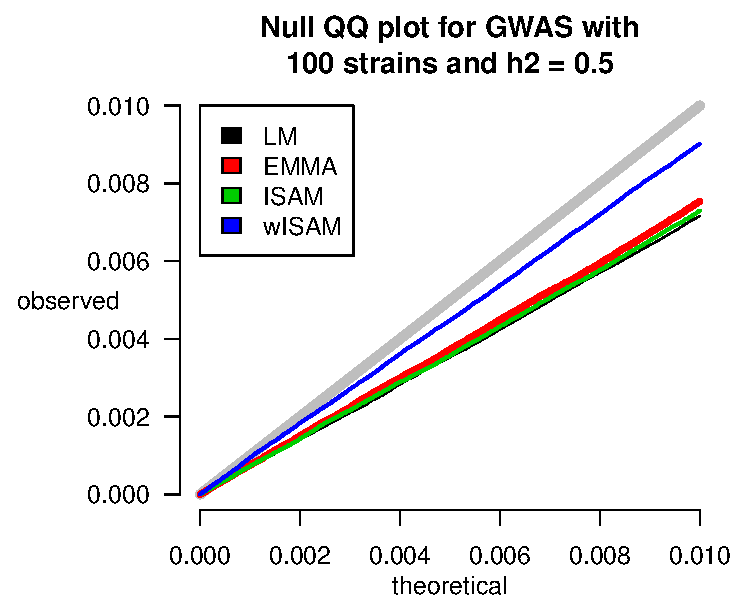
\includegraphics[width = 0.5\textwidth]{images/exampleQQ.pdf}
  \caption[
    Example quantile-quantile (QQ) plot.
  ]
  {
    This quantile-quantile (QQ) plot of the $p$ values from all four tests shows that they all are anti-conservative and that the weighted ISAM, the only method to use $\bM_\text{het}$ is the least anti-conservative.
  }
  \label{fig:exampleQQ}
\end{figure}

For example, the simulation with 100 organisms and $h^2 = 0.5$ showed that all four tests are anti-conservative and that the weighted ISAM, the only method to use $\bM_\text{het}$ is the least anti-conservative (\autoref{fig:exampleQQ}).
The QQ plot shown in \autoref{fig:exampleQQ} is zoomed to the range [0, 0.01] in both the theoretical (horizontal) and realized (vertical) axis.
I show the rest of the QQ plots with increasing zoom from the range [0, 1] to the range [0, 0.001] to show both the global behavior and the behavior in the zone that really matters for large scale analysis, the very small $p$ values.
Given the large number of hypotheses that are tested in a GWAS and the multiple hypothesis testing corrections that must be made to account for the large number of hypotheses, the most relevant $p$-value cutoffs to evaluate are the very small ones.

\autoref{fig:qqmegaplot1}, \autoref{fig:qqmegaplot2}, and \autoref{fig:qqmegaplot3} show the behavior of all four tests across all simulation scenarios.
Some consistent patterns emerge.

First, the higher the heritability and the larger the strain panel, the more anti-conservative is the LM.
In the most extreme case (\autoref{fig:qqmegaplot3}, row 4, column 5), the observed $p$-values rise less than a hundredth of distance they are expected to over the interval [0, 0.001].
Practically speaking, this observation implies that there is one $p$ value less than 0.001 out of every 10 tests, though should only be one out of every 1,000 tests.
This pattern is present to varying degrees in traits with $h^2 \in {0.7, 0.9}$ for all panel sizes.

Second, there is never any meaningful difference between EMMA and my unweighted ISAM implementation.
This is consistent with a correct implementation, as these tests are theoretically identical.

Third, the EMMA and ISAM tests are overly-conservative when applied to traits with low heritability, especially when few strains are used.
The most extreme observation of this behavior can be seen in \autoref{fig:qqmegaplot1}, row 4, column 1.
The observed $p$ values reach the top of the plot about half way across, indicating that there is one $p$ value less than 0.001 every approximately every 20,000 tests, though there should be one every 10,000 tests.
This pattern is present to varying degrees for traits with $h^2 \in {0.1, 0.3}$ in a panel with 50 or 100 strains and for a trait with $h^2 = 0.1$ in a panel of 200 organisms.

Finally, the EMMA and ISAM tests are anti-conservative when applied to traits with high heritability when few strains are used.
In the most extreme case (\autoref{fig:qqmegaplot1}, row 4, column 5), the observed $p$-values rise about half the distance they are expected to over the interval [0, 0.001].
This pattern indicates that there are two $p$-values less than 0.001 out of every 1,000 tests, while there should be only one.
Said another way, there is one $p$-value less than 0.001 for every 5,00 tests, while there should be one every 1,000 tests.
The weighted ISAM, the only test that uses $\bM_\text{het}$ rather than $\bM_\text{hom}$ rises to about three quarters of its expected height, indicating that there are about 1.5 $p$-values less than 0.001 out of every 1,000 tests, while there should be only one.
This behavior is still not ideal, as there should be only 1 $p$-value less than 0.001 out of every 1,000 tests, but it is closer to ideal than the EMMA and ISAM tests, which use $\bM_\text{hom}$.

\begin{sidewaysfigure}
  \centering
  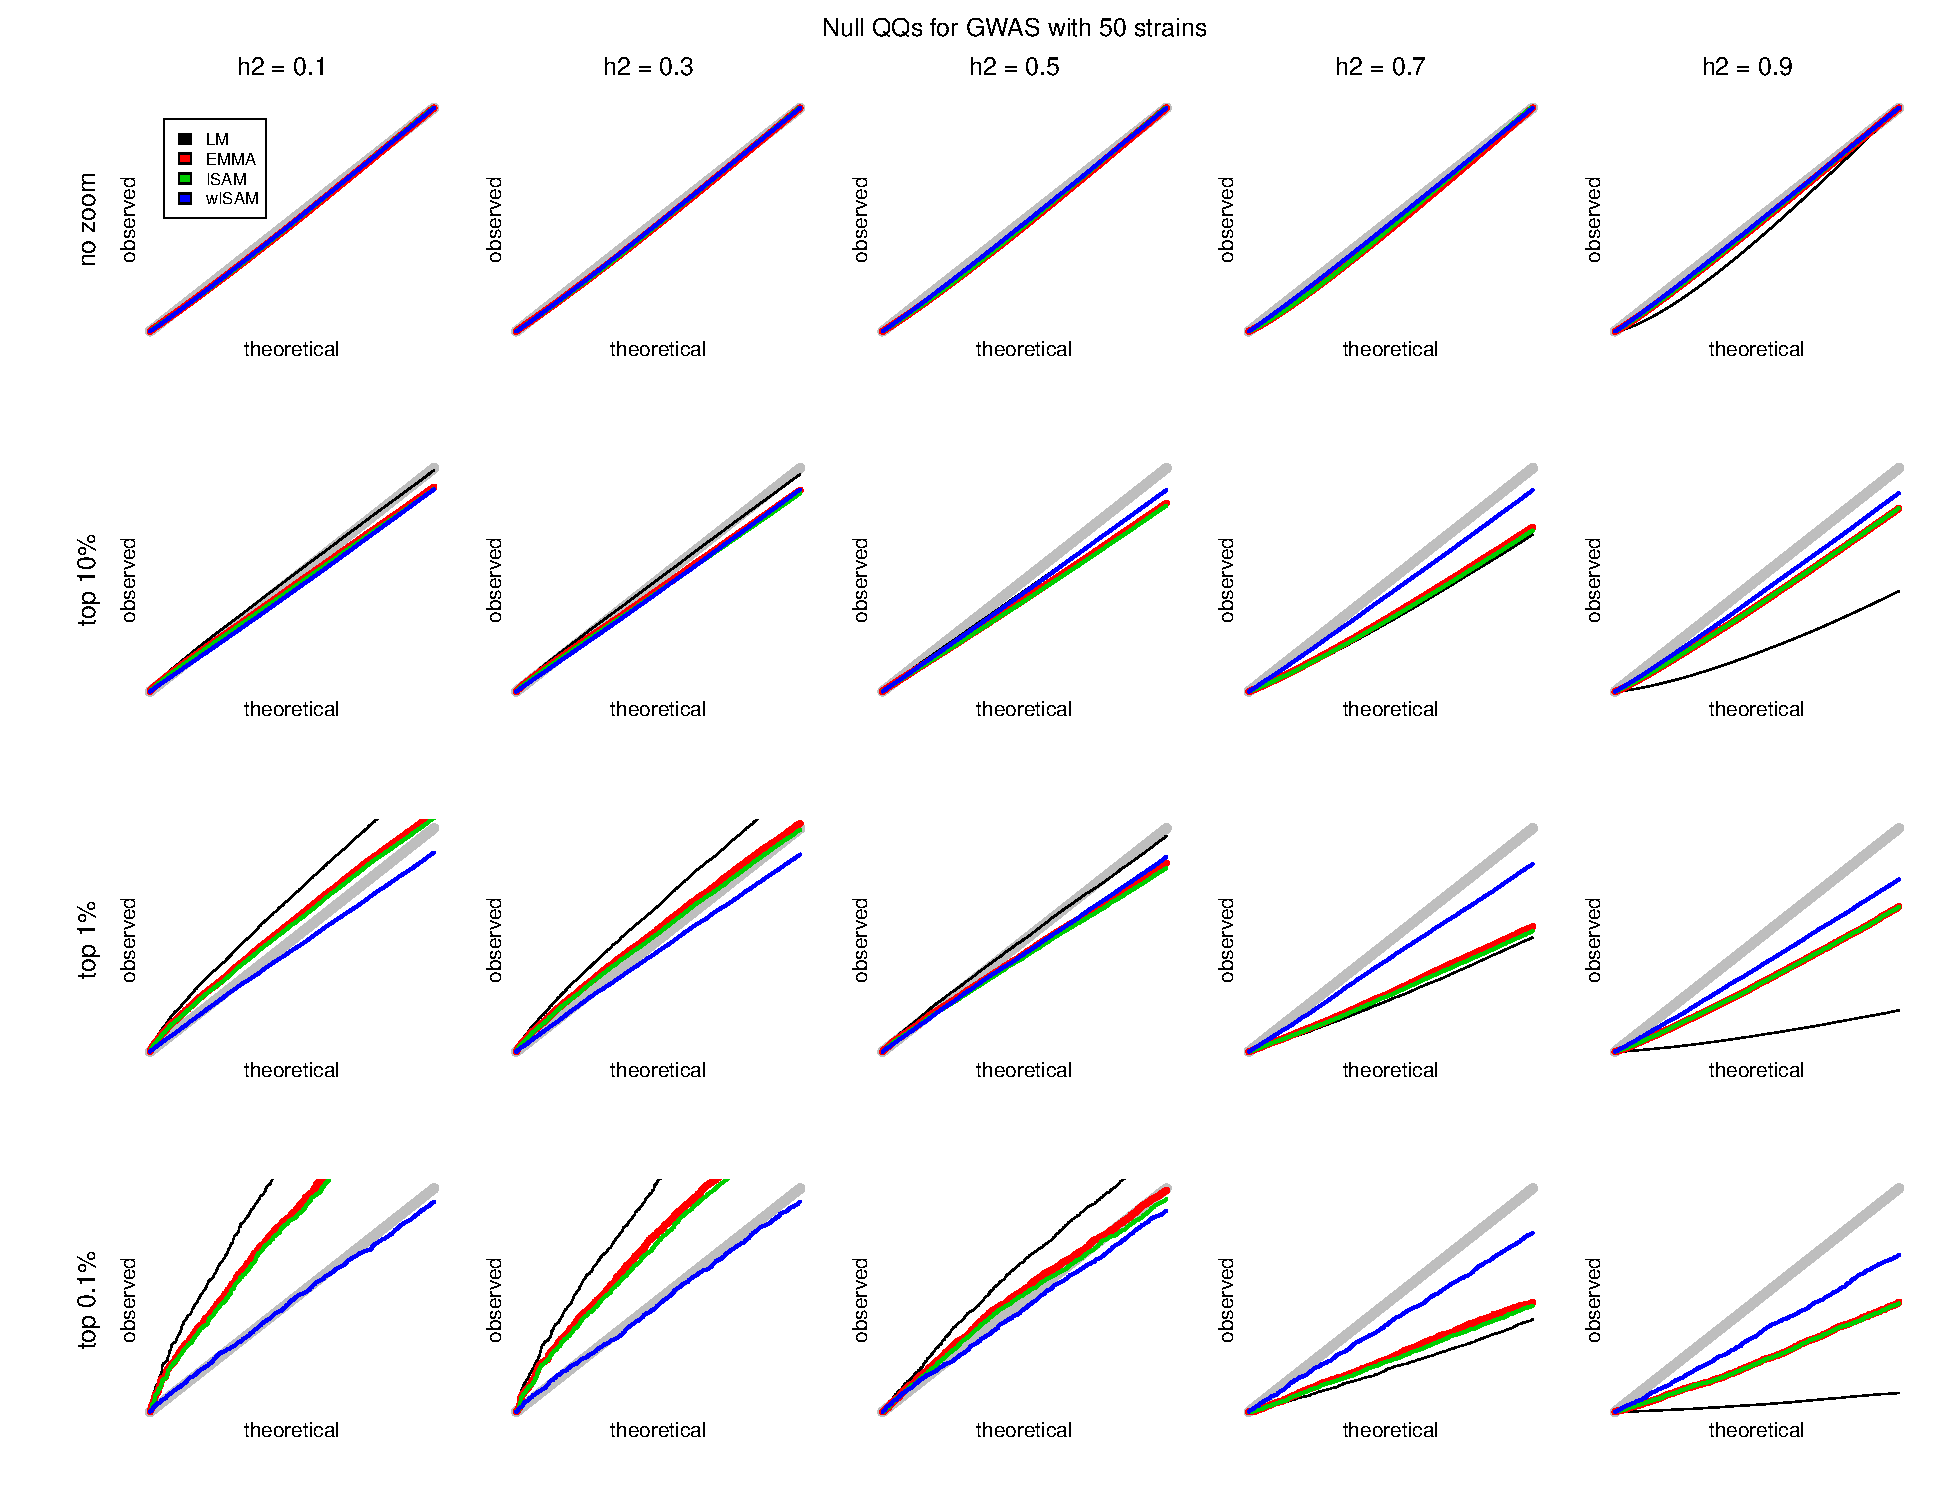
\includegraphics[width = 0.9\textwidth]{images/2018-05-19alt_heterosked_sims_nstrain=50_nsnps=100_nsims=10000.pdf}
  \caption[
    QQ plots for simulations with 50 organisms in the mapping panel.
  ]{
    QQ plots for simulations with 50 organisms (or strains) in the mapping panel.
    Heritability increases from left to right and zoom increases from top to bottom.
    For traits with low and very low heritability (0.1 and 0.3), wISAM is uniquely resistant to overly conservative behavior.
    For traits with high and very high heritability (0.7 and 0.9), wISAM is uniquely resistant to anti-conservative behavior.
    For traits with heritability of 0.5, all tests have nearly-accurate FPR control.
  }
  \label{fig:qqmegaplot1}
\end{sidewaysfigure}

\begin{sidewaysfigure}
  \centering
  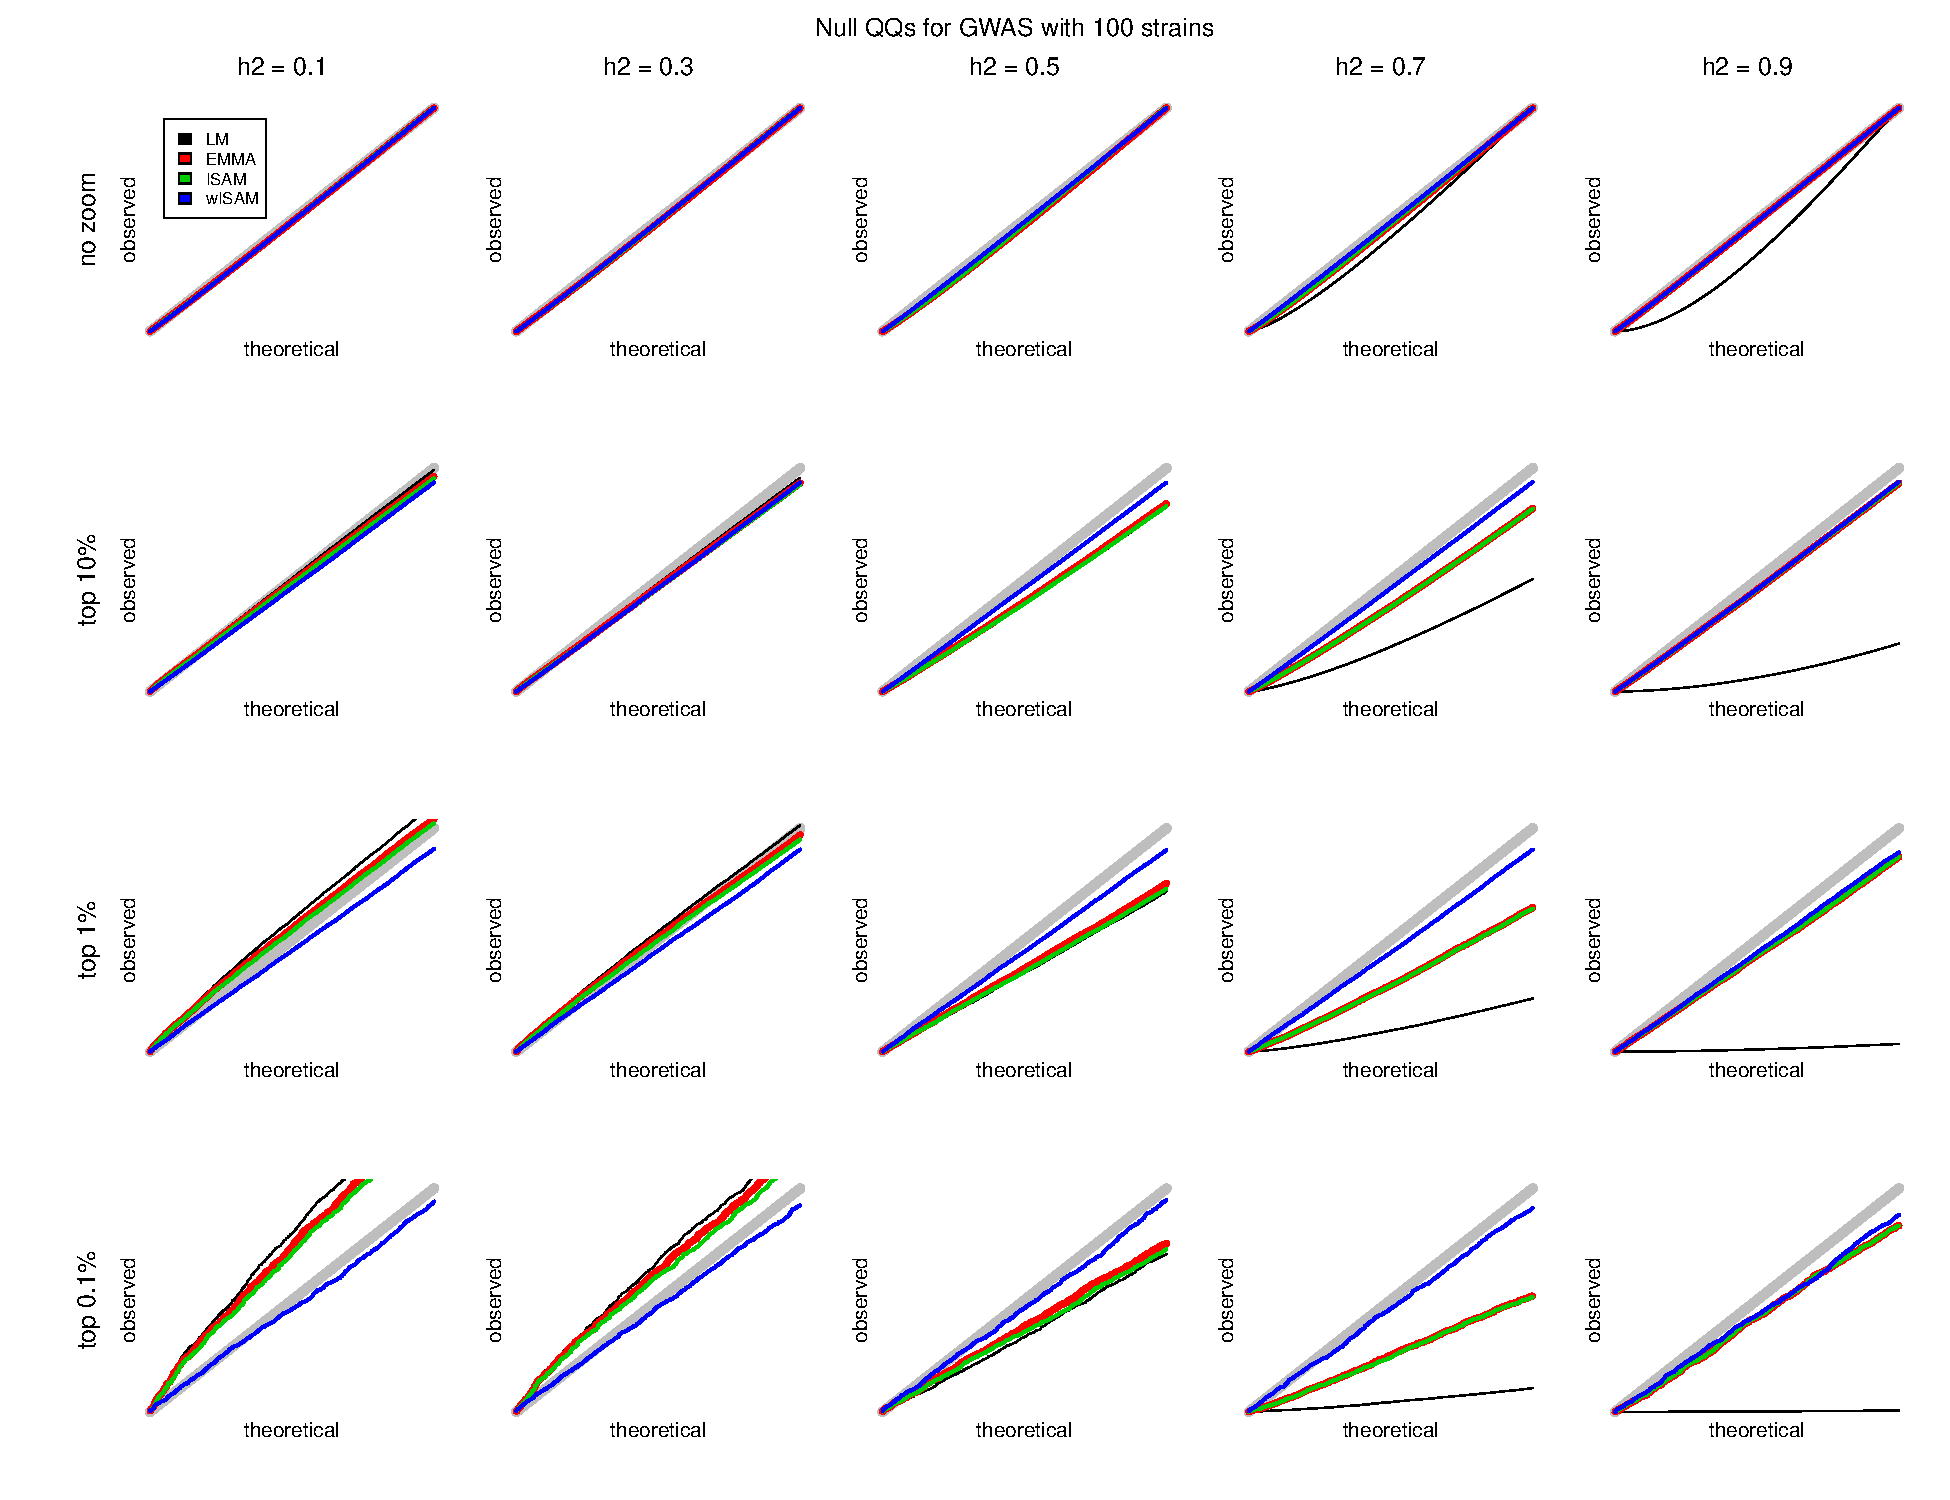
\includegraphics[width = 0.9\textwidth]{images/2018-05-19alt_heterosked_sims_nstrain=100_nsnps=100_nsims=10000.pdf}
  \caption[
    QQ plots for simulations with 100 organisms in the mapping panel.
  ]{
    QQ plots for simulations with 100 organisms (or strains) in the mapping panel.
    Heritability increases from left to right and zoom increases from top to bottom.
    For traits with low and very low heritability (0.1 and 0.3), wISAM is uniquely resistant to overly conservative behavior.
    For traits with moderate and high heritability (0.5 and 0.7), wISAM is uniquely resistant to anti-conservative behavior.
    For traits with heritability of 0.9, all LMM-based tests have nearly-accurate FPR control.
  }
  \label{fig:qqmegaplot2}
\end{sidewaysfigure}

\begin{sidewaysfigure}
  \centering
  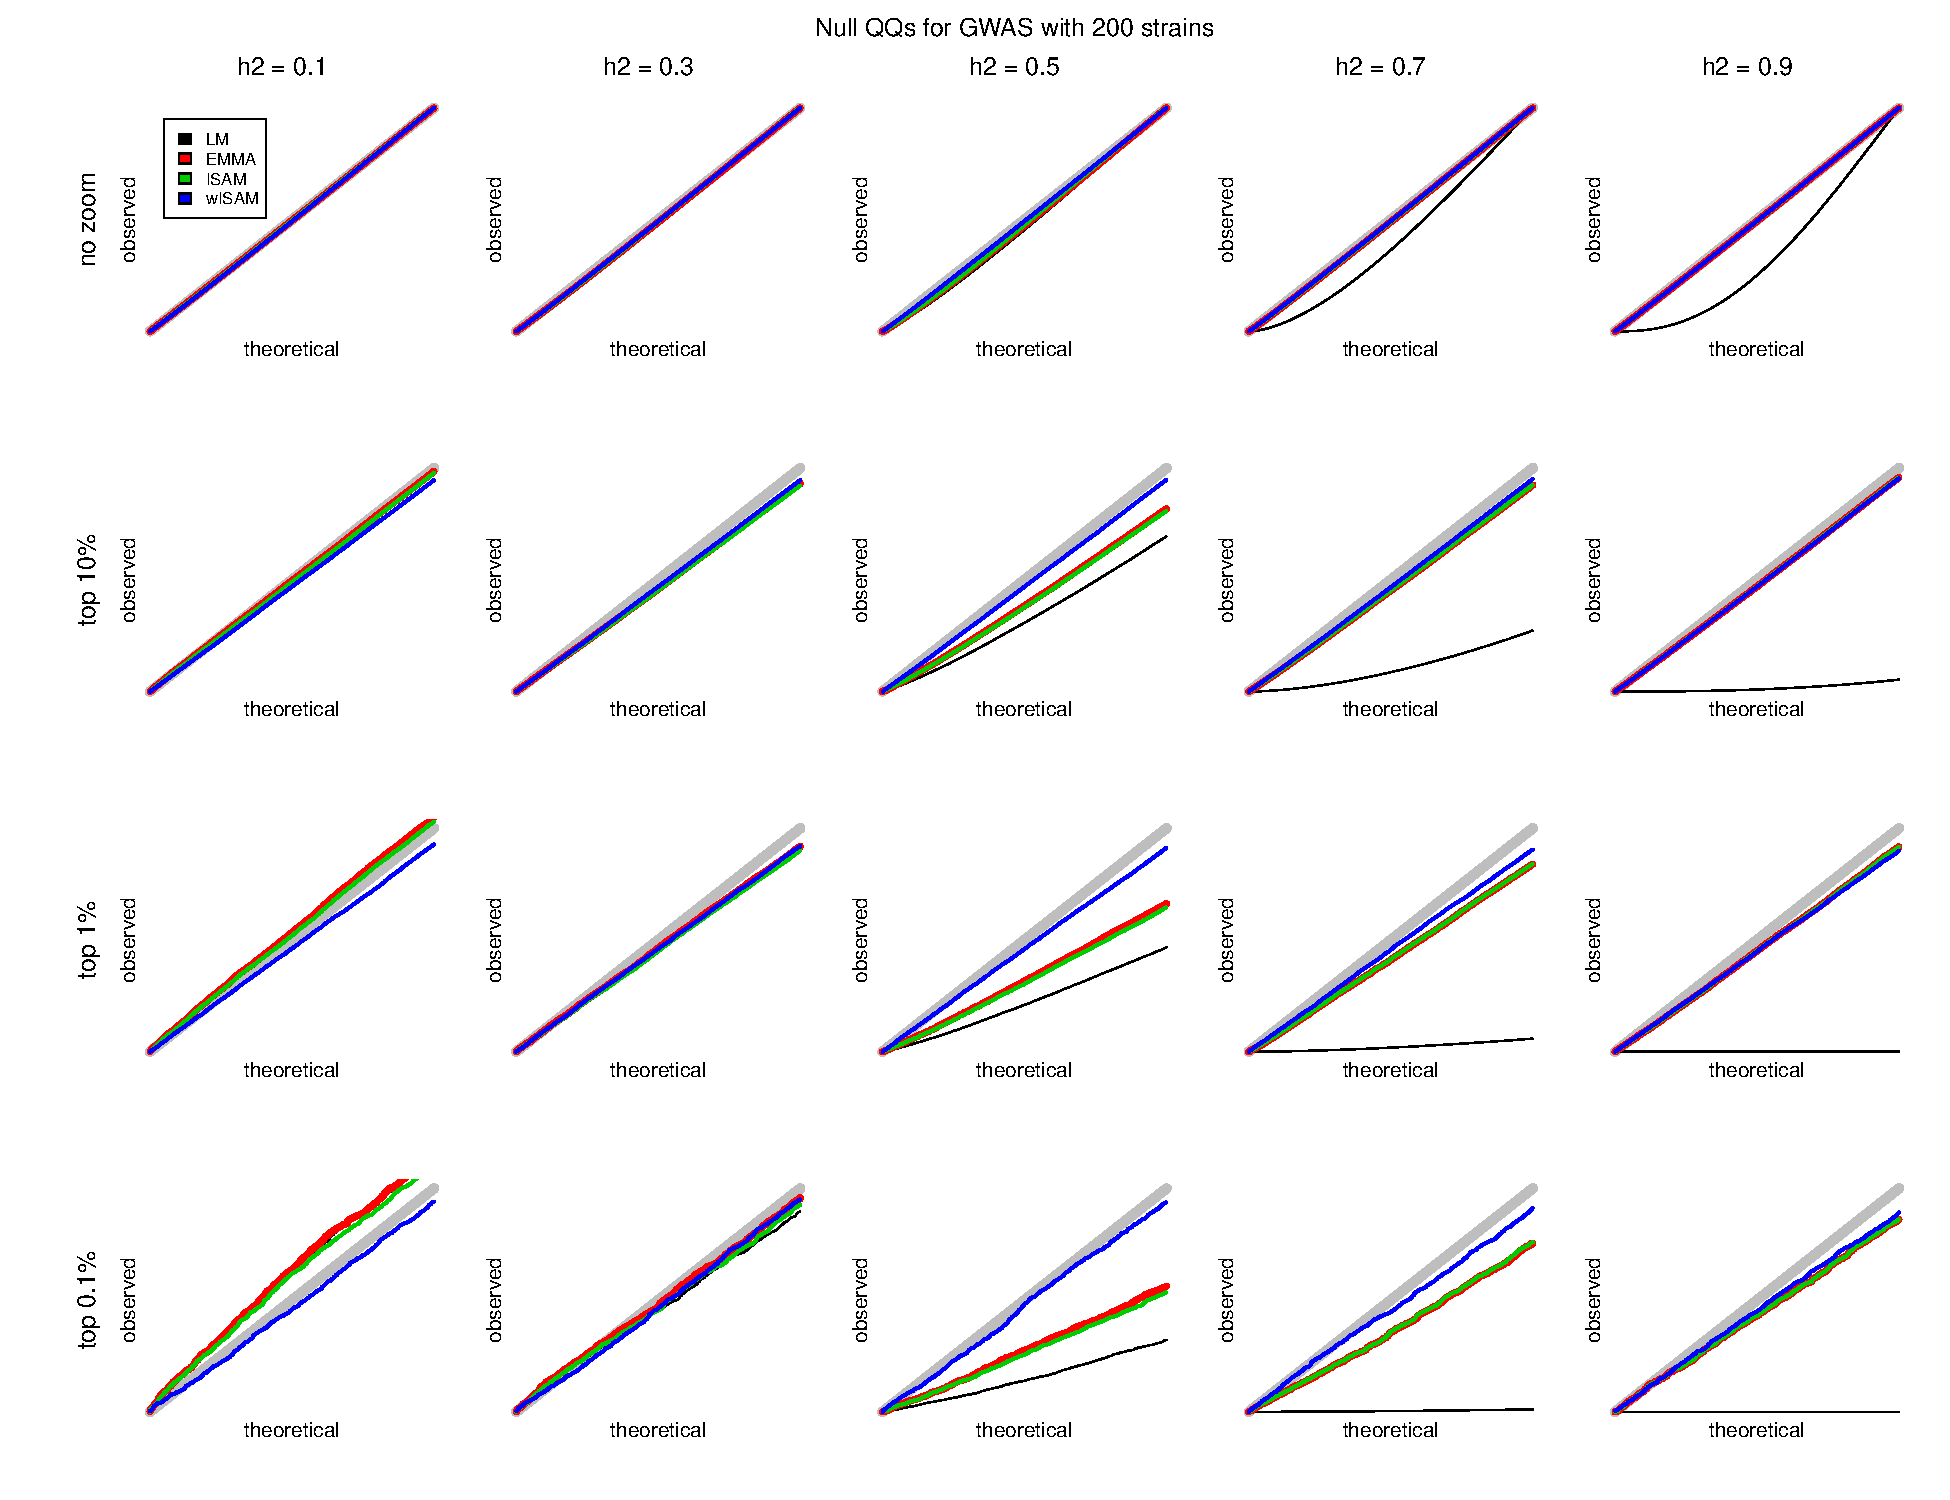
\includegraphics[width = 0.9\textwidth]{images/2018-05-19alt_heterosked_sims_nstrain=200_nsnps=100_nsims=10000.pdf}
  \caption[
    QQ plots for simulations with 200 organisms in the mapping panel.
  ]{
    QQ plots for simulations with 200 organisms (or strains) in the mapping panel.
    Heritability increases from left to right and zoom increases from top to bottom.
    For traits with heritability of 0.1, wISAM is uniquely resistant to overly conservative behavior.
    For traits with heritability of 0.3, all tests have nearly-accurate FPR control.
    For traits with moderate to high heritability (0.5 to 0.7), wISAM is uniquely resistant to anti-conservative behavior.
    For traits with heritability of 0.9, all LM-based tests have nearly-accurate FPR control.
  }
  \label{fig:qqmegaplot3}
\end{sidewaysfigure}


\subsection{Discrimination between real and spurious signals}

Another important way to evaluate the behavior of the tests to compare their ability to discriminate real from spurious signals.
Where FPR control under the null used only null simulations, this evaluation combines information from null and alternative simulations.
To compare the discrimination of weighted and unweighted LMM-based tests, I compared their receiver operating characteristic (ROC) curves.

This method of evaluation involves collecting test statistics from both null and alternative data and calculating, for each possible cutoff, the true positive rate and the false positive rate.
For a cutoff, $c$, the true positive rate is the fraction of alternative that have a test statistic greater than the cutoff.
Similarly, the false positive rate is the fraction of null simulations that have a test statistic greater than the cutoff.

Two points are guaranteed to be in every ROC plot.
If $\inf$ is used as the cutoff, no tests will be called positive, so both the true positive rate and the false positive rate will be 0 and thus (0, 0) is on every ROC curve.
If $-\inf$ is used as the cutoff all tests will be called positive, so both the true positive rate and the false positive rate will be 1 and thus (1, 1) is on every ROC curve.
For a test with no ability to discriminate between null and alternative simulations, the ROC curve progresses from (0, 0) to (1, 1) along a straight line with slope 1.
For a test that perfectly discriminates between null and alternative simulations, the ROC curve progresses directly up from (0, 0) to (0, 1) and then directly to the right to (1, 1).
Most tests have intermediate discrimination ability, between random guessing and perfect, so their ROC curve progresses through the upper left portion of the plot.
The closer the ROC curve is to that of a perfect test, the better the test.

ROC analysis exploring the entire parameter space describe for the FPR control under the null has not yet been completed.
Here, I show the ROC curve that resulted for a study with $h^2 = 0.5$ and 100 organisms, the middle-of-the-road parameter set \autoref{fig:exampleROC}.
\begin{figure}
  \centering
  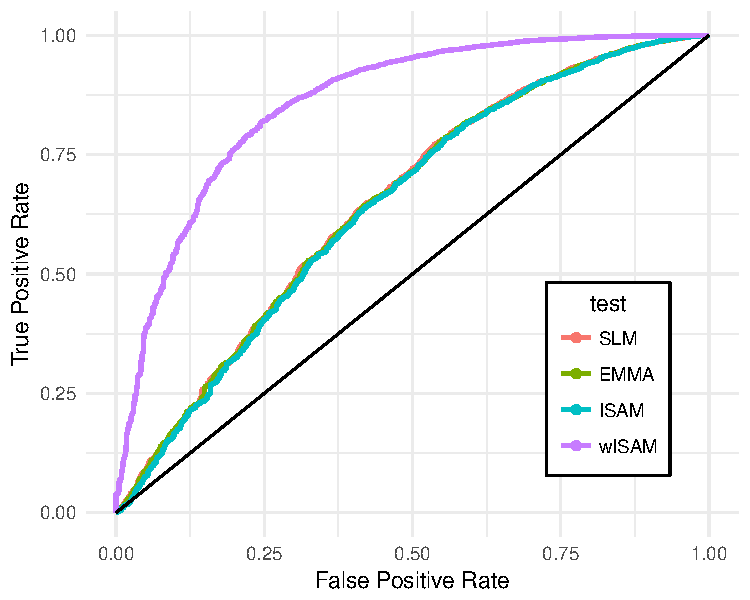
\includegraphics[width = 0.5\textwidth]{images/roc_hetsked_100snps_1ksims_05h2_100strains.pdf}
  \caption[
    Receiver operating characteristics (ROC) curve for a GWAS with 100 organisms on a trait with $h^2 = 0.05$.
  ]
  {
    Receiver operating characteristics (ROC) curve for a GWAS with 100 organisms on a trait with $h^2 = 0.05$.
    The ROC curve for the weighted ISAM is superior to that of the other LMM-based methods and the LM.
  }
  \label{fig:exampleROC}
\end{figure}


\section{Software}

I implemented a linear mixed model fitter that can handle heteroskedastic residual variance using the method described in this chapter.
This software is freely available on github at \url{https://github.com/rcorty/wISAM} and on CRAN at \url{CRANURL}.